
\chapter{Superhydrophobic Droplet Impact - Comparison with Gerris simulations}

\section{Contact angle}
\begin{wrapfigure}{r}{0.5\textwidth}
  \begin{center}
    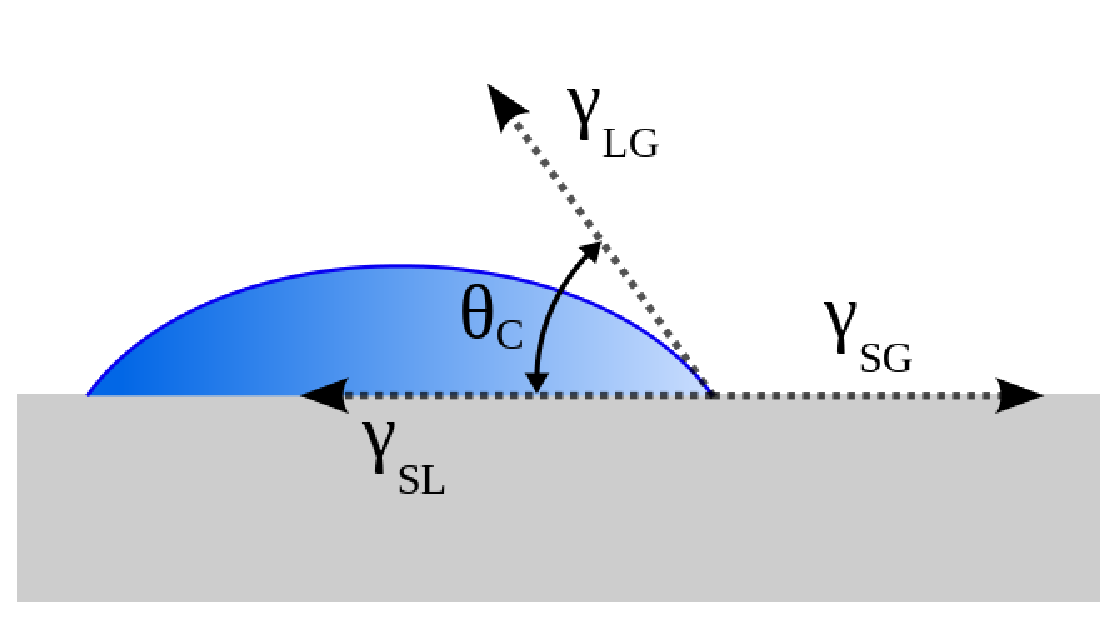
\includegraphics[width=0.48\textwidth]{Contact_angle.eps}
  \end{center}
  \caption{Contact Angle}
  \label{Fig:Contact_angle}
\end{wrapfigure}
When a gas-liquid interface meets a solid surface, at the point of contact of three phases the liquid makes an angle with the surface. This measures the wettability of 
the solid surface for that liquid. The contact angle is given by Young's equation, ( See Figure \ref{Fig:Contact_angle} ). 
\begin{equation}
 \boxed{ \begin{align}
 &\gamma_{SG} -\gamma_{SL} - \gamma_{LG} \cos \theta =0  \\
 &\cos \theta =\frac{\gamma_{SG} -\gamma_{SL}}{\gamma_{LG}} 
 \end{align}
 }
 \label{Eq:youngs}
\end{equation}
which expresses the balance of forces acting on the contact line in the direction normal to the contact line and tangential
to the solid surface. Experiments show that the contact angle deviates from its static value when
the contact line is in motion. This deviation is an important feature of the problem and needs to be taken into account to obtain realistic answers.\\
\underline{\textbf{Superhydrophobic surfaces}}\par
The effect of the dynamic contact angle and moving contact line however can be made minimal if the spreading of the droplet is very less. Such phenomenon is seen in non-wetting surfaces. 
Surfaces which are extremely difficult to wet are known as superhydrophobic surfaces. \cite{wang2007definition} has attempted to define the superhydrophobic surfaces as the
surfaces that exhibit static contact angle greater than $150^o$. In the next sections we compared some experimental studies on superhydrophobic surfaces with simulations done on Gerris.
% \begin{figure}
% \centering
%     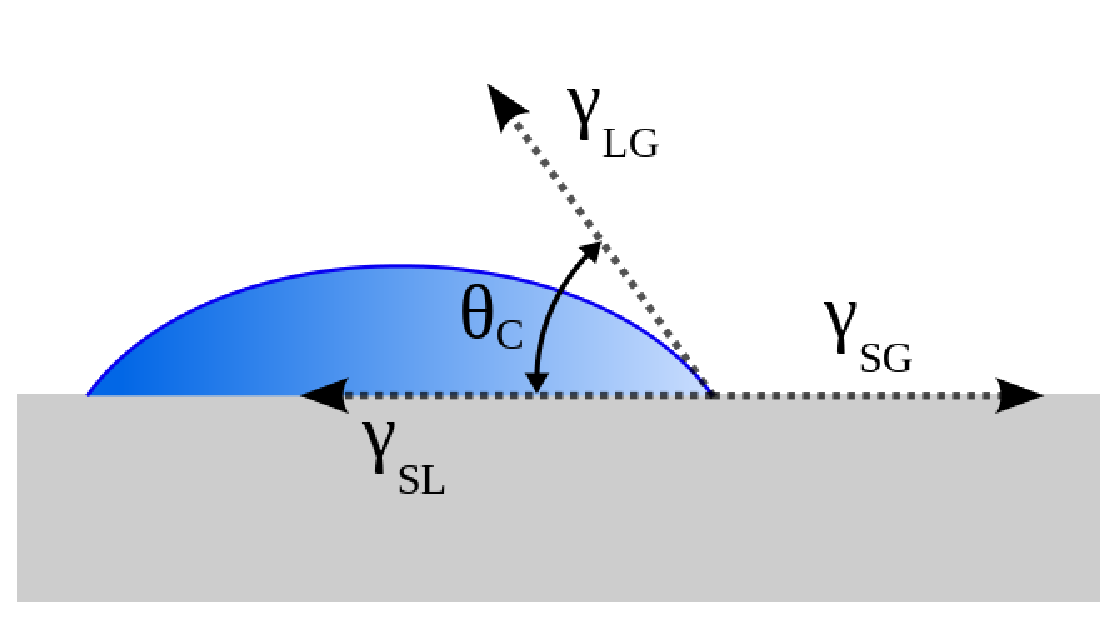
\includegraphics[width=0.48\textwidth]{Contact_angle.eps}
%   \caption{Contact angle}
%   \label{Fig:Contact_angle}
% \end{figure}

\section{Gerris}
Gerris is an open source code created by \cite{Popinet2003} which solves Navier stokes equation using a VOF method for constructing the interface.
\begin{equation}
 \boxed {\begin{align}
 \frac{d \tilde u}{d\tilde t} &= \frac{1}{\rho_k} \left\{ - \tilde \nabla p + \frac{1}{Re_L}  \tilde \nabla \cdot ( \mu_k (\tilde \nabla \tilde u + \nabla \tilde u^T )) 
 + \frac{1}{We_L} \kappa \delta_s \overrightarrow n \right\} + \frac{1}{Fr^2} \\
 \tilde \nabla . \tilde u &= 0 \qquad\text{(Equation of continuity)}\\
 \frac{D\tilde F}{D\tilde t}&=0 \qquad\text{(Volume of Fluid advection equation)}
\end{align} }
\label{Eq:gerris_nd}
\end{equation}
where, 
 \begin{table}[H]
  \begin{center}
   \caption{Variables symbols}
 \label{variables}
    \begin{tabular}{ll}
      \toprule 
	  Variable & Remark   \\ 
	  \midrule
	  $\rho_L$ & Density of liquid  \\ 
	    $\rho_g$ & Density of gas \\
	    $\mu_L$ & Viscosity of liquid  \\
	    $\mu_G$ & Viscosity of gas \\
	     $\frac{\rho_G}{\rho_L}$ & Density ratio gas to liquid \\
	    $\frac{\mu_L}{\mu_L}$ & Viscosity ratio gas to liquid  \\
	    $\sigma_{LG}$ & Surface tension of Liquid-gas   \\
	    $D$ & Diameter of the droplet  \\
	    $g$ & Acceleration due to gravity \\
      \bottomrule \\
    \end{tabular}
  \end{center}
\end{table}
 
\begin{equation*}
\begin{align}
&Re_L = \frac{\rho_L D U}{\mu_L}  &\textbf{(Reynolds Number)}\\
&We_L = \frac{\rho_L D U}{\mu_L}  &\textbf{(Weber Number)}\\ 
&Fr = \frac{U}{\sqrt{gD}}  &\textbf{(Froude Number)}\\
\end{align}
\end{equation*}

The primary current limitation of Gerris flow solver is it does not have \textbf{Dynamic Contact Angle (DCA)} model. In order to find out if lack of dynamic contact angle model affects 
droplet spreading on superhydrophobic surfaces, we compare Gerris simulation with experimental data from \cite{Hung2011}, \cite{Clanet2004} and \cite{Wang2007}
having no-slip conditions and static contact angle at the surface.

\subsection{Simulations}

The problems studied for comparison has the parameters given in Table \ref{parameters} \\

 \begin{table}[H]
  \begin{center}
    \begin{tabular}{ccccccc}
      \toprule 
      Author(s) & $Re_L$ & $We_L$ & $Fr$ & $\rho_k$ & $\mu_k$ & Contact Angle \\ 
      \midrule
      \cite{Hung2011} & 2521 & 29 & 5 & $2 X 10^{-3}$ &  $2 X 10^{-2}$ & $150^{\circ}$ \\
       \cite{Clanet2004} & 2327 & 24 & 5 & $2 X 10^{-3}$ &  $2 X 10^{-2}$ & $170^{\circ}$ \\
        \cite{Wang2007} & 1256 & 9 & 4 & $2 X 10^{-3}$ &  $2 X 10^{-2}$ & $163^{\circ}$\\
      \bottomrule \\
    \end{tabular}
       \caption{Input to solver}
 \label{parameters}
  \end{center}
\end{table}

\underline{Boundary Conditions}: No slip conditions on all walls except axis of symmetry where we use symmetry conditions (described in section \ref{sec:bc}). Impact surface
has a static contact angle.
\subsubsection{\textbf{Gerris simulation vs \cite{Hung2011}}}
\begin{figure}
 \centering
 \subfloat[t = 0.0357 ]{%
      \includegraphics[width=0.3\textwidth]{hung-1.eps}
      }
  \subfloat[t = 0.0361 ]{%
      \includegraphics[width=0.3\textwidth]{hung-2.eps}
      } 
       \subfloat[t = 0.0362 ]{%
      \includegraphics[width=0.3\textwidth]{hung-3.eps}
      }\\
       \subfloat[t = 0.0365 ]{%
      \includegraphics[width=0.3\textwidth]{hung-4.eps}
      }
    \subfloat[t = 0.0368 ]{%
      \includegraphics[width=0.3\textwidth]{hung-5.eps}
      }
       \subfloat[t = 0.0371 ]{%
      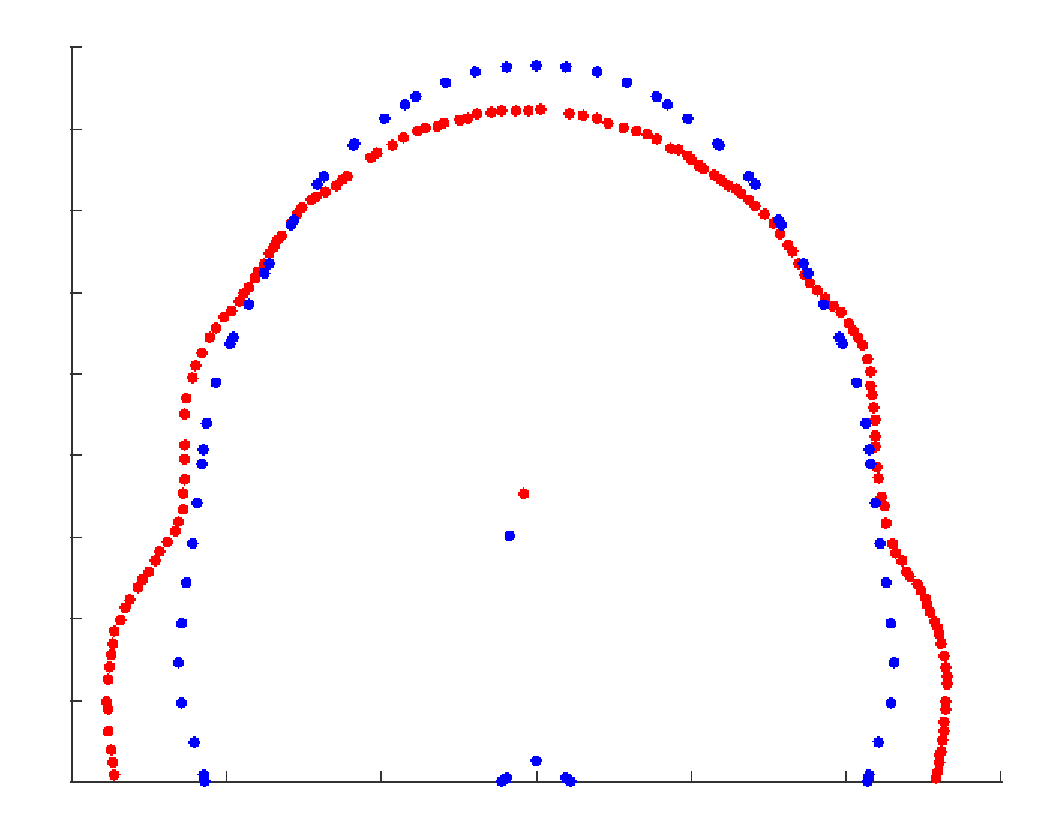
\includegraphics[width=0.3\textwidth]{hung-6.eps}
      }\\
       \subfloat[t = 0.0374 ]{%
      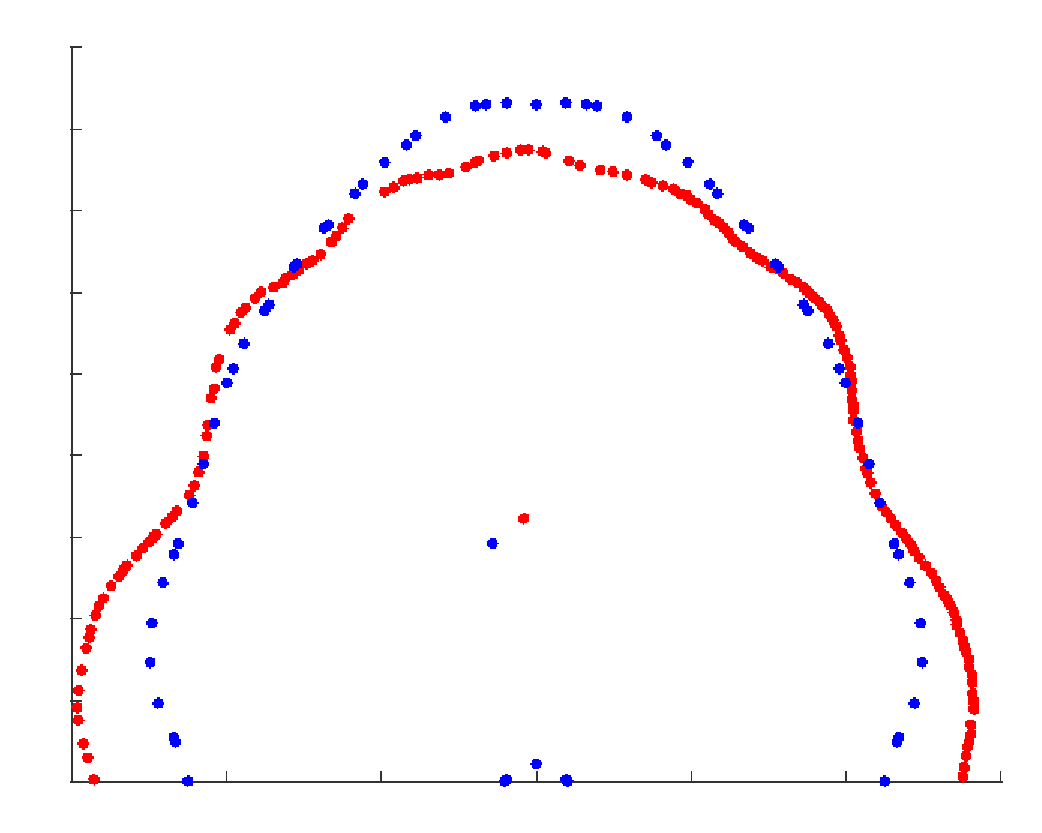
\includegraphics[width=0.3\textwidth]{hung-7.eps}
      }
       \subfloat[t = 0.0377 ]{%
      \includegraphics[width=0.3\textwidth]{hung-8.eps}
      }
       \subfloat[t = 0.0379 ]{%
      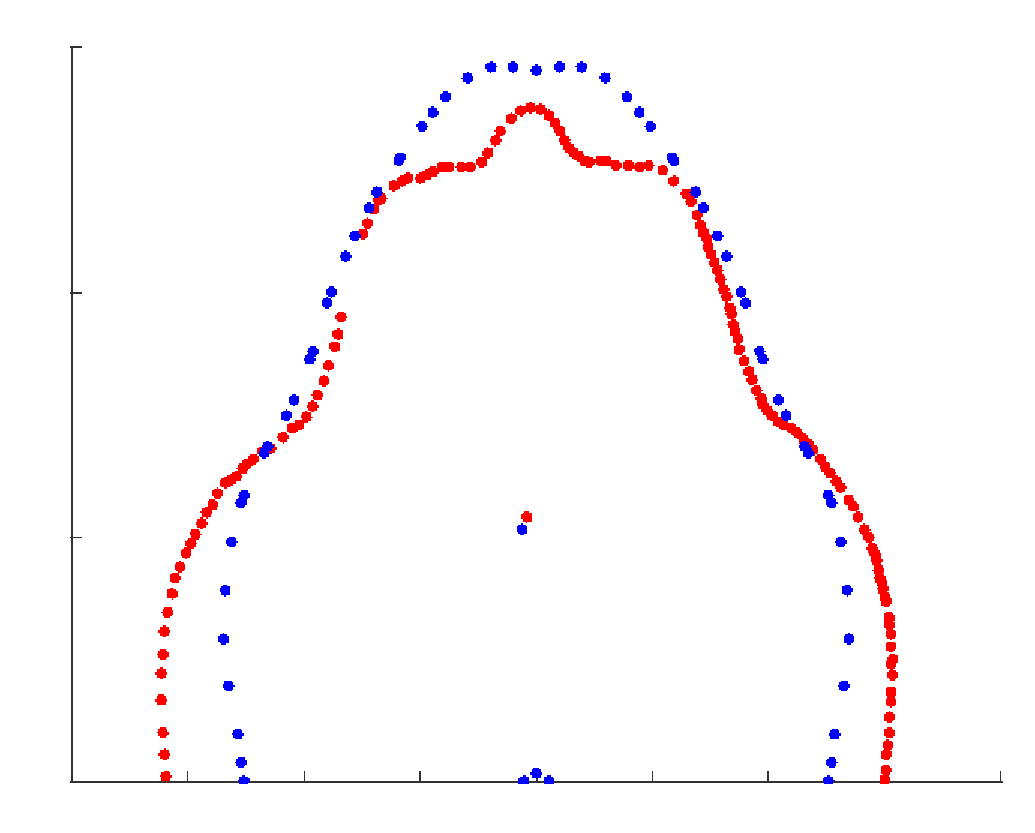
\includegraphics[width=0.3\textwidth]{hung-9.eps}
      }\\
%        \subfloat[t = 0.0382 ]{%
%       \includegraphics[width=0.3\textwidth]{hung-10.eps}
%       }
 \caption{Interface and center of mass Gerris simulation data(blue) with \cite{Hung2011} experimental data(red), Contact Angle $150^o$}
 \label{Fig:gs5}
 \end{figure}

The interface points and center of mass from the experimental data (\cite{Hung2011}) were extracted and compared with Gerris simulation data. 
The simulation results are seen to be in agreement with experiments before impact. Just after impact (See Figure \ref{Fig:gs5} (a),(b)) the contact line and the contact angle coincides with 
the experimental data but as the contact line starts to move, the simulation interface does not move because of the no slip boundary condition. From (c) to (i) it is seen that
the results are somewhat different from what is observed in the experiment. The vertical position of center of mass is less sensitive to the impact surface.
Figure \ref{Fig:y_com} shows the variation of vertical height of center of mass of droplet with respect to time. It looks like a damped oscillation.

\subsubsection{\textbf{Gerris simulation vs \cite{Clanet2004}}}
\begin{figure}[H]
 \centering
 \subfloat[t = 26.2 ]{%
      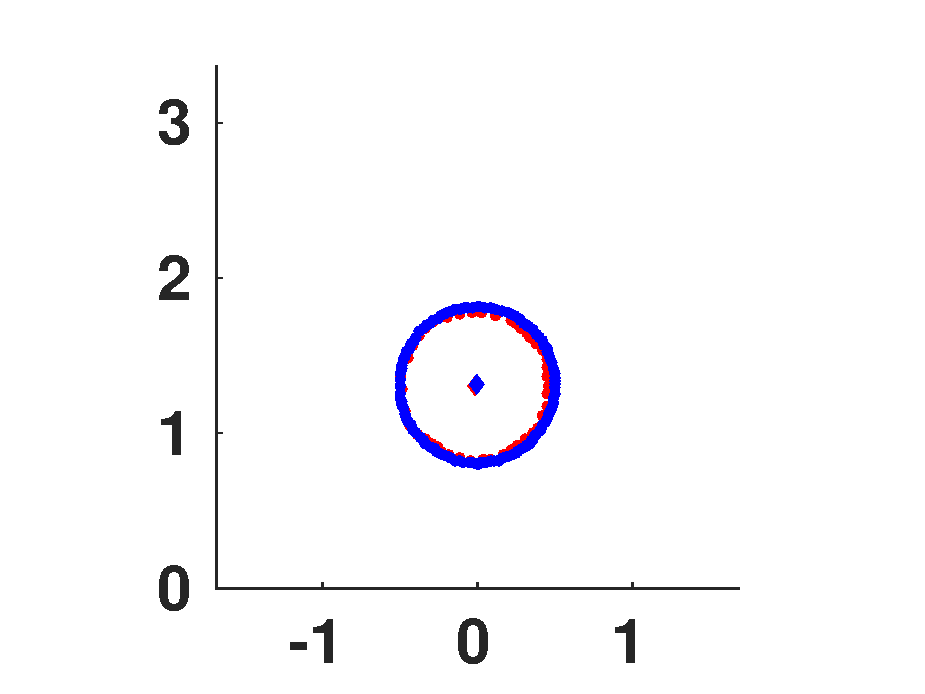
\includegraphics[width=0.3\textwidth]{clanet-1.eps}
      }
  \subfloat[t = 27.1 ]{%
      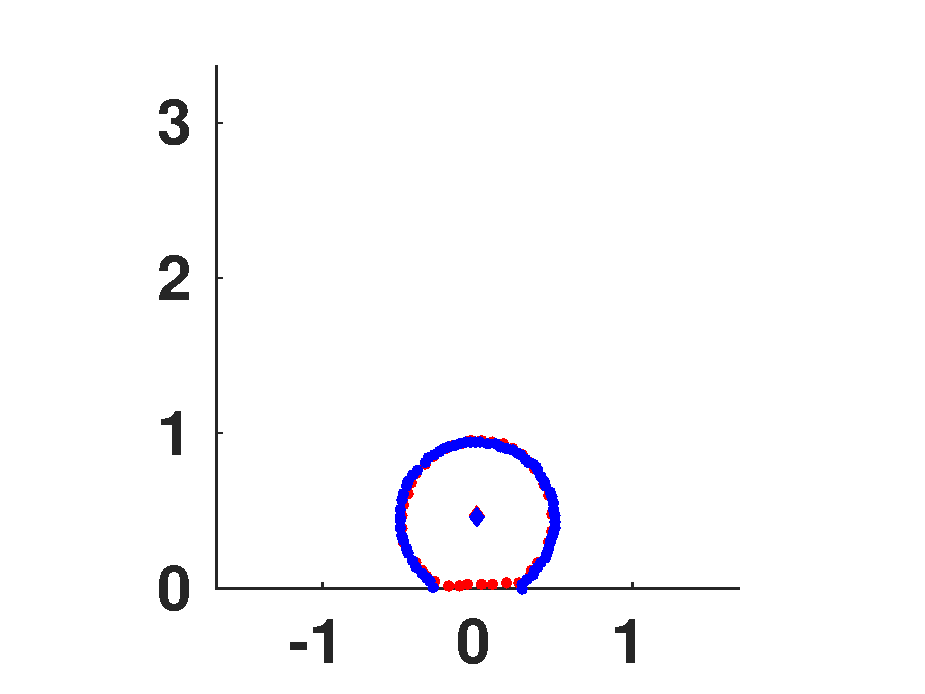
\includegraphics[width=0.3\textwidth]{clanet-2.eps}
      } 
       \subfloat[t = 28.0 ]{%
      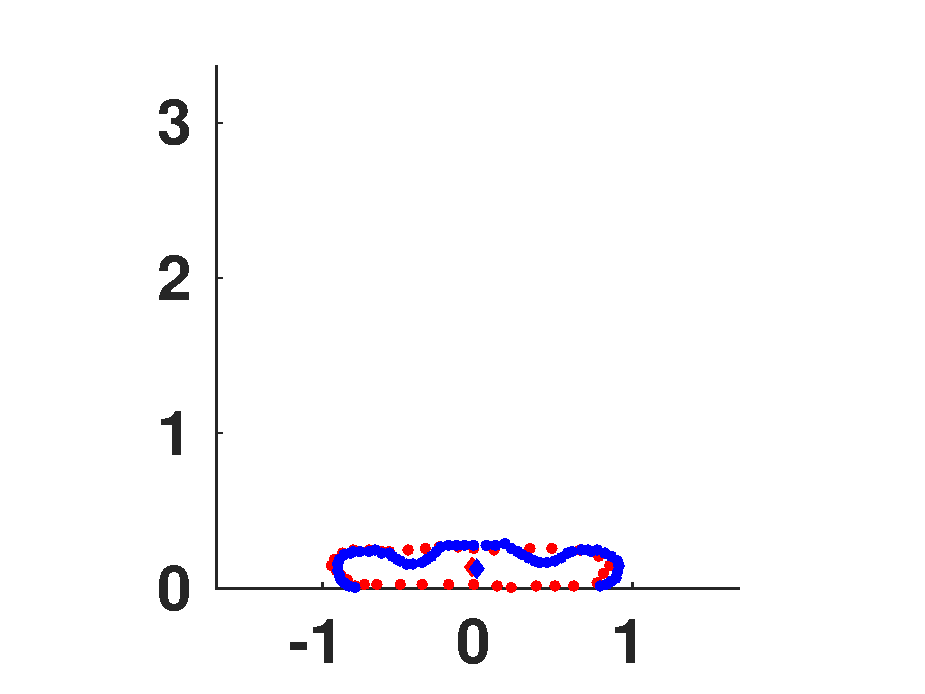
\includegraphics[width=0.3\textwidth]{clanet-3.eps}
      }\\
       \subfloat[t = 28.9 ]{%
      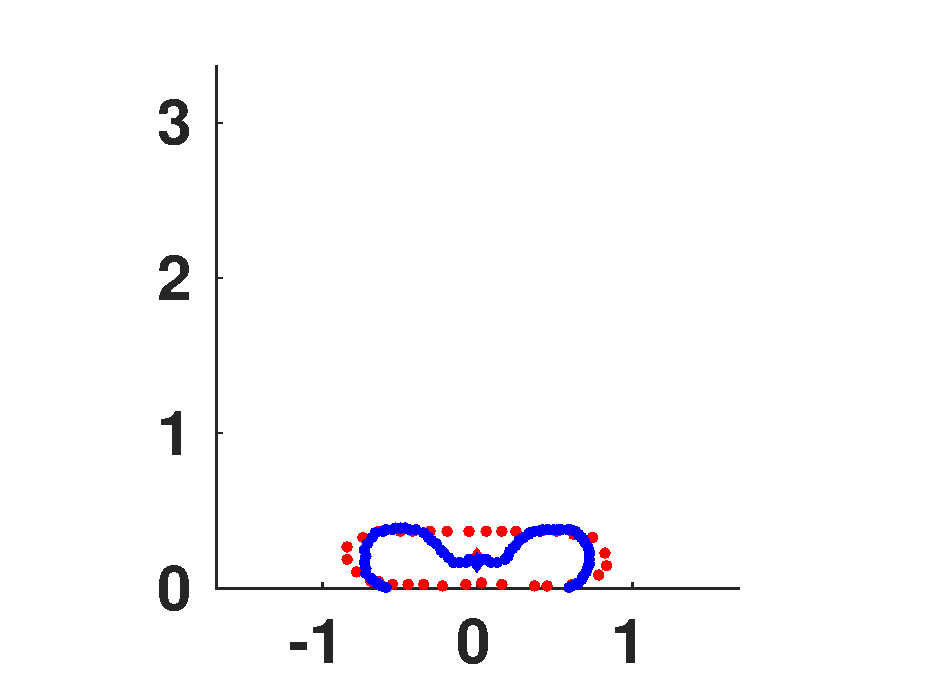
\includegraphics[width=0.3\textwidth]{clanet-4.eps}
      }
    \subfloat[t = 29.8 ]{%
      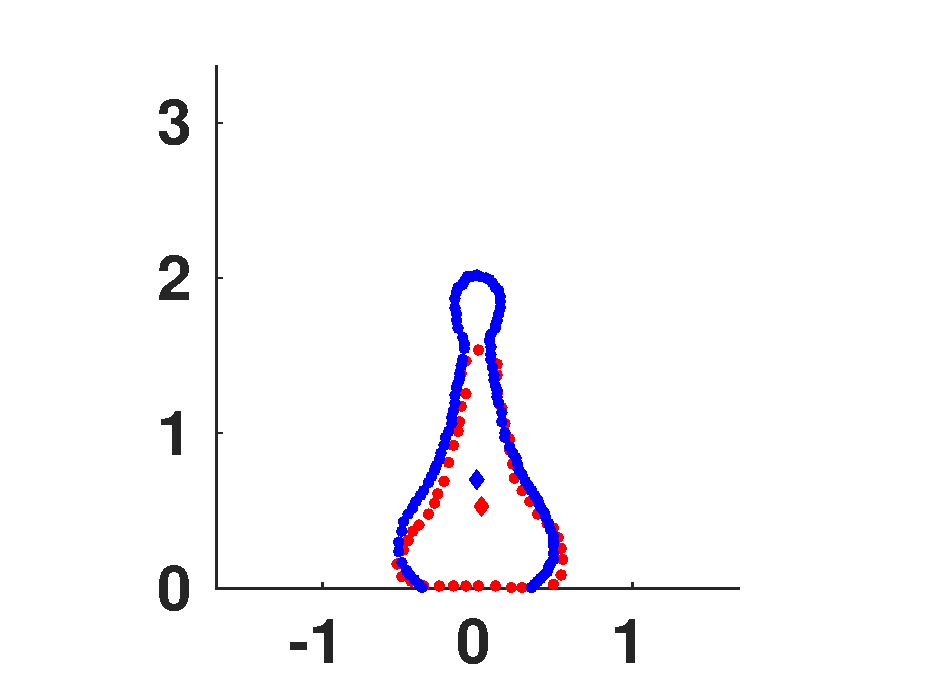
\includegraphics[width=0.3\textwidth]{clanet-5.eps}
      }
       \subfloat[t = 30.7 ]{%
      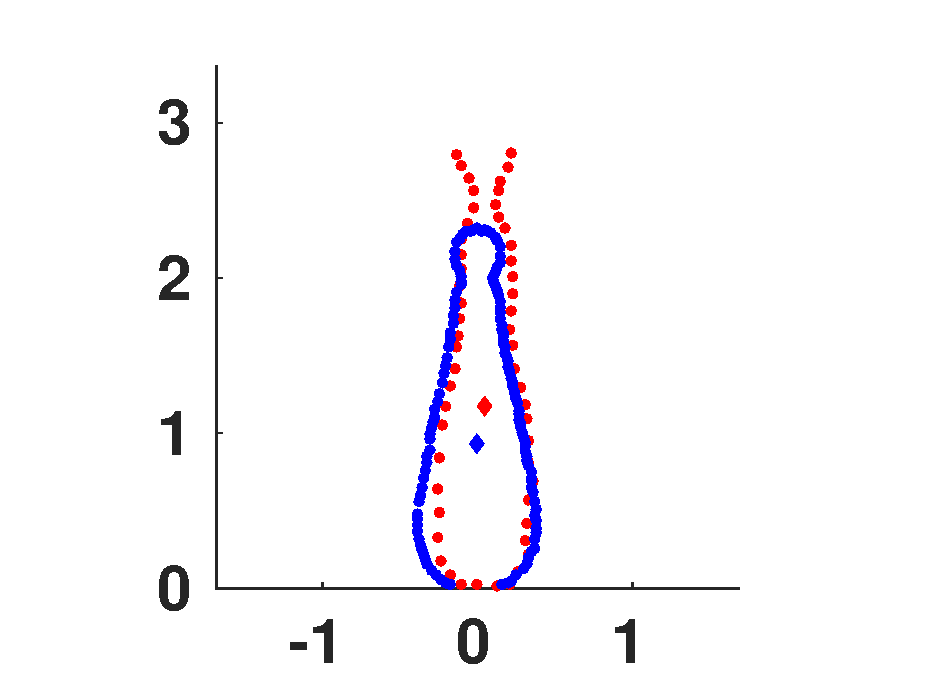
\includegraphics[width=0.3\textwidth]{clanet-6.eps}
      }\\
       \subfloat[t = 31.6 ]{%
      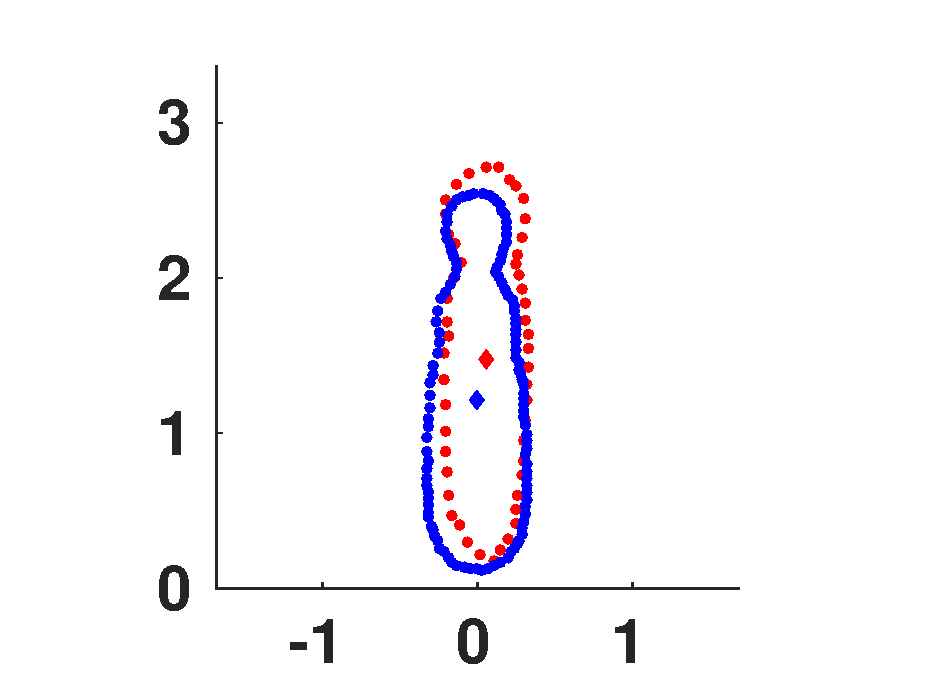
\includegraphics[width=0.3\textwidth]{clanet-7.eps}
      }
       \subfloat[t = 32.5 ]{%
      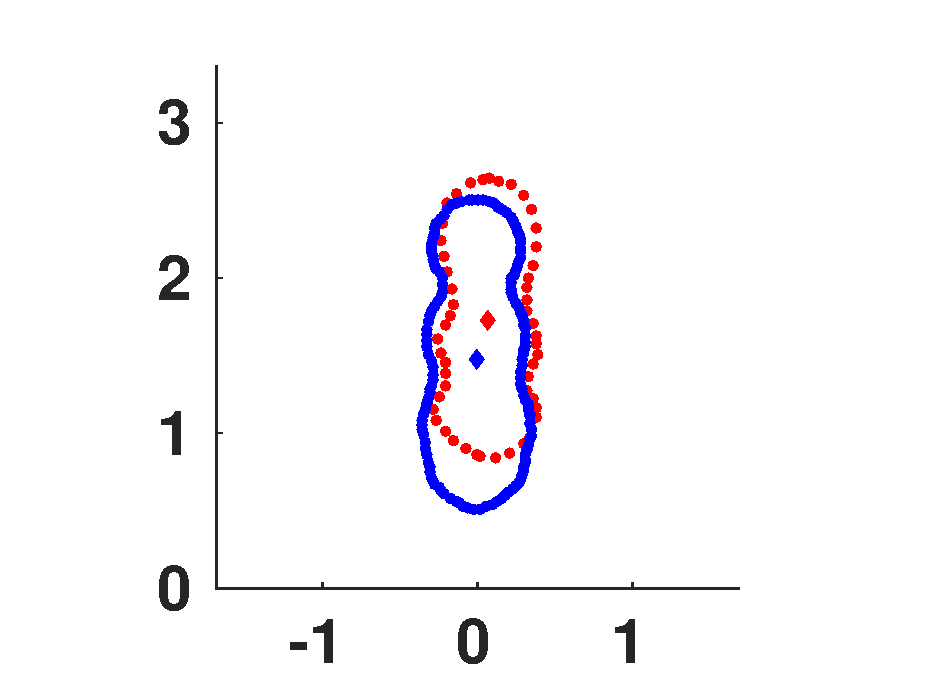
\includegraphics[width=0.3\textwidth]{clanet-8.eps}
      }
       \subfloat[t = 33.4 ]{%
      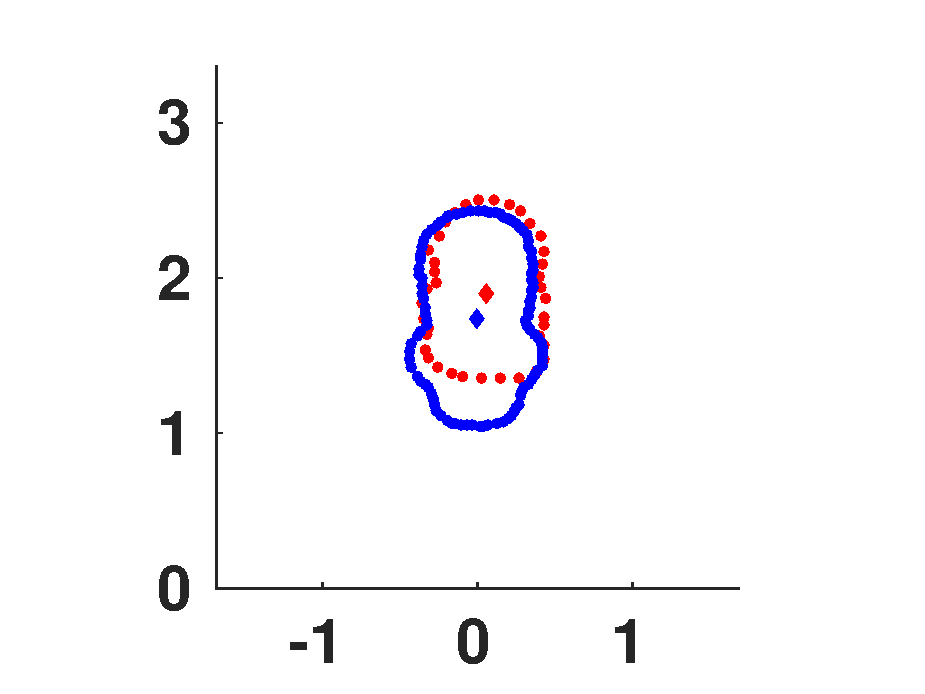
\includegraphics[width=0.3\textwidth]{clanet-9.eps}
      }
 \caption{Interface Gerris simulation data(blue) with \cite{Clanet2004} experimental data(red) Contact Angle $170^o$}
 \label{Fig:gs6}
 \end{figure}
  \cite{Clanet2004} showed that droplet impacting on superhydrophobic surfaces behaves like a balloon filled with fluid in some regime of parameters,
 where the movement of contact line is restricted and the boundary condition for velocity can be taken as no-slip. 
 This study involved superhydrophobic surfaces with contact angle of  $170^o$. We made a comparison with Gerris simulation with static contact angle
 boundary condition and no slip  at surface (See Figure \ref{Fig:gs6} and \ref{Fig:y_com_clanet}). It can be seen that superhydrophobic surfaces has very little
 spreading and has minimal effect on 
 the dynamics of droplet impact.
  \begin{figure}[H]
  \centering
 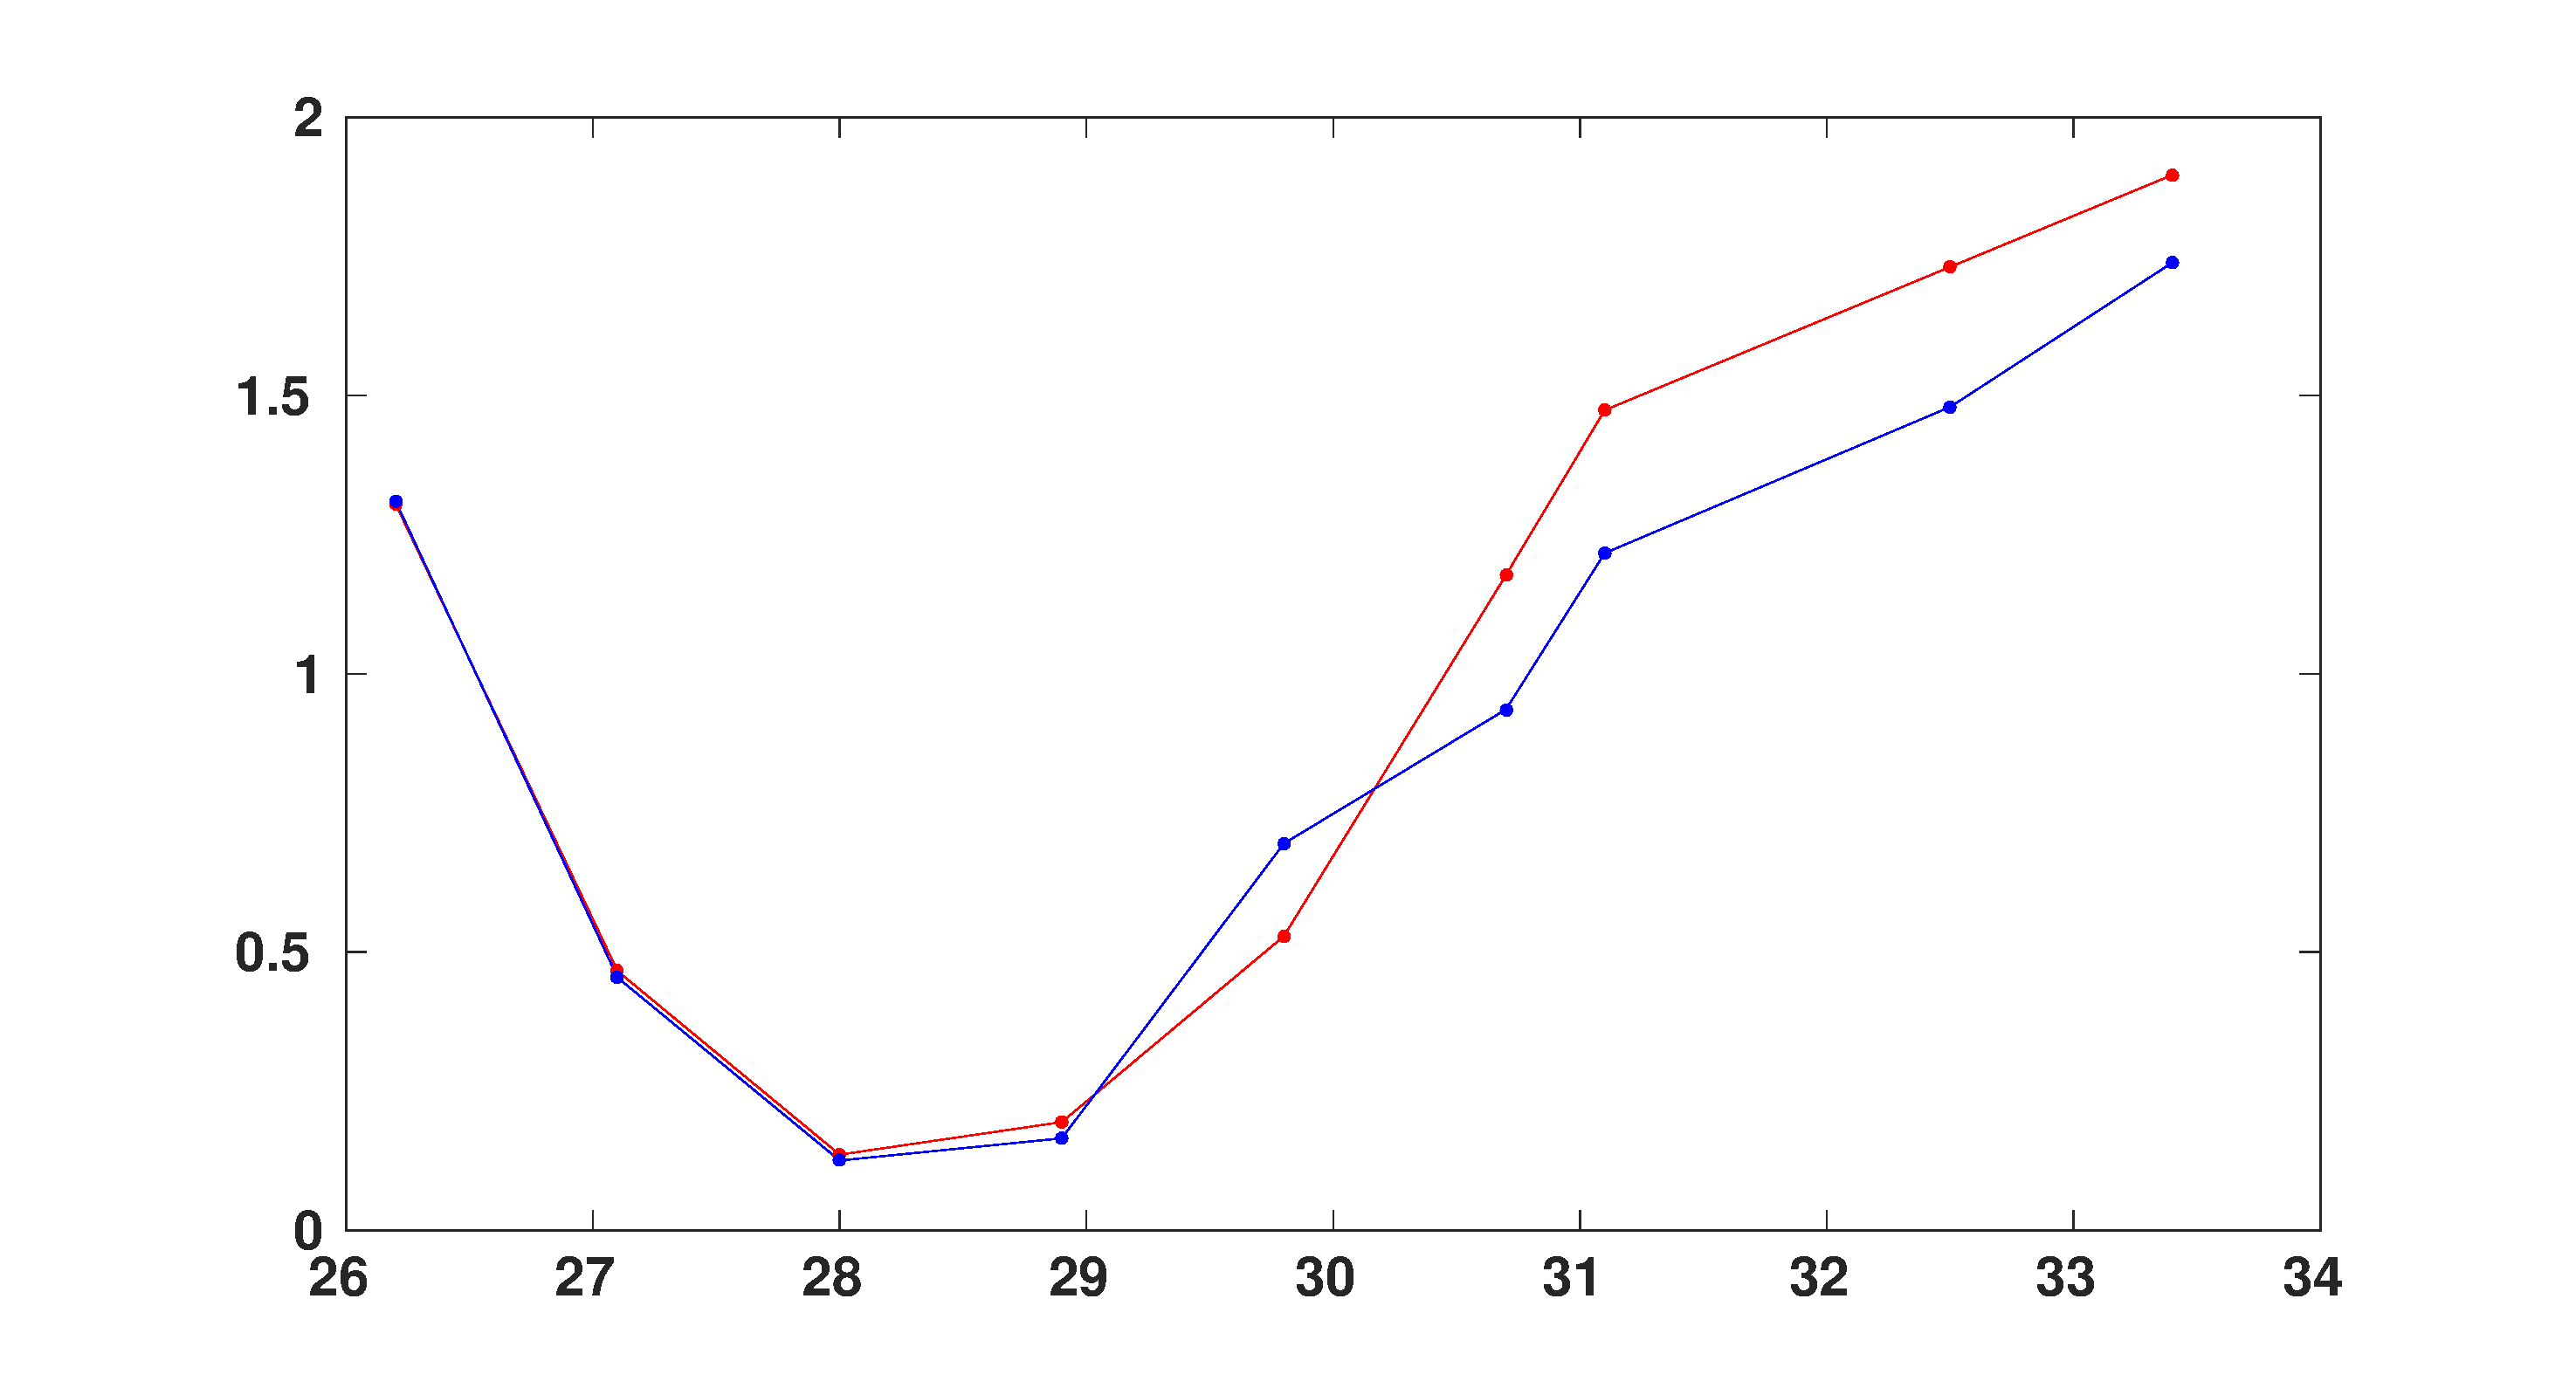
\includegraphics[scale=0.2]{y_com_clanet.eps}
 \caption{y coordinate of center of mass of droplet to time. blue-Gerris, red-\cite{Clanet2004}}
 \label{Fig:y_com_clanet}
\end{figure}

 \subsubsection{\textbf{Gerris simulation vs \cite{Wang2007}}}
 A comparison with \cite{Wang2007} (See Figure \ref{Fig:gs7}), the surface has a contact angle of $163^o$, also corroborate the fact that the static contact angle conditions
are a good approximation for the solution of droplet impact on superhydrophobic surfaces.\\

 \begin{figure}[H]
 \centering
 \subfloat[t = 15.6 ]{%
      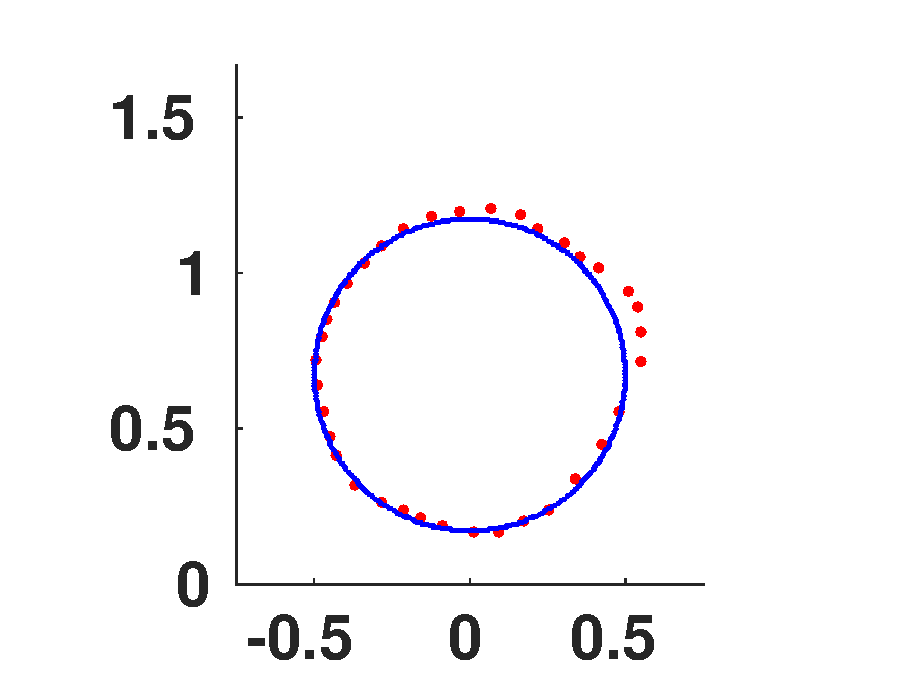
\includegraphics[width=0.3\textwidth]{wang-1.eps}
      }
  \subfloat[t = 16.0 ]{%
      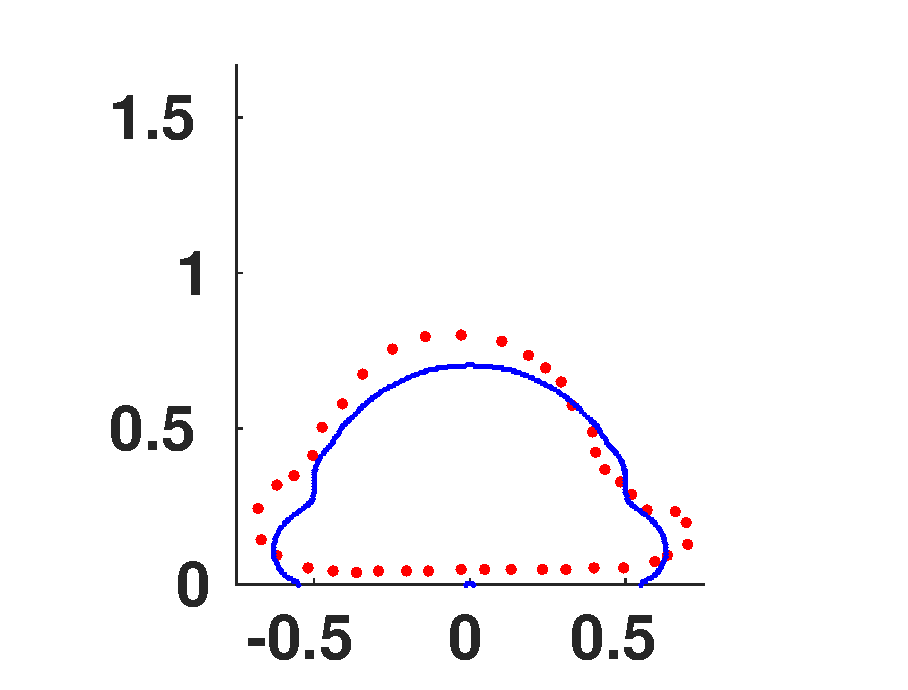
\includegraphics[width=0.3\textwidth]{wang-2.eps}
      } 
       \subfloat[t = 17.0 ]{%
      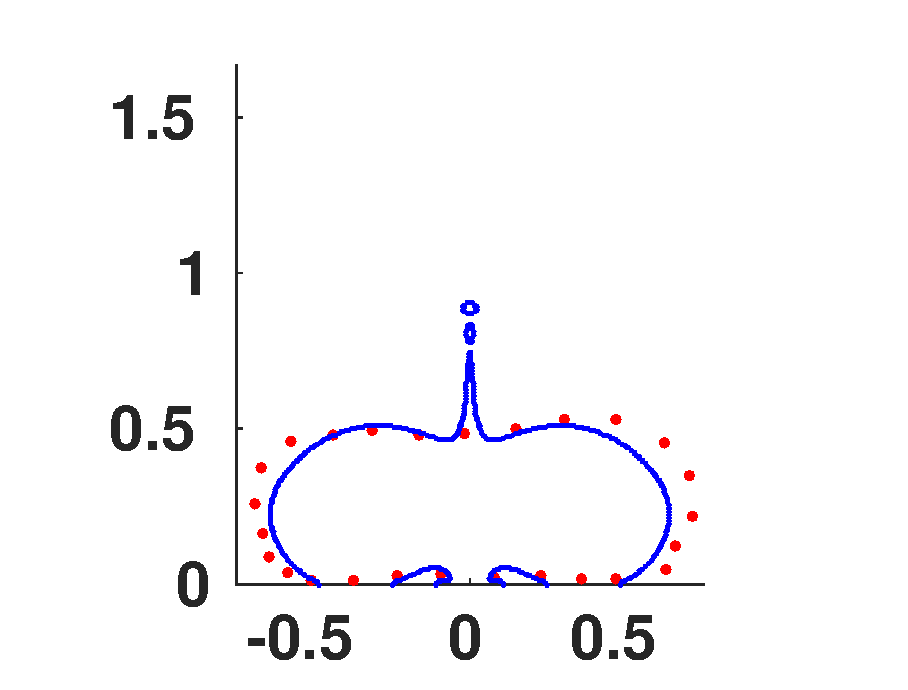
\includegraphics[width=0.3\textwidth]{wang-3.eps}
      }\\
       \subfloat[t = 18.1 ]{%
      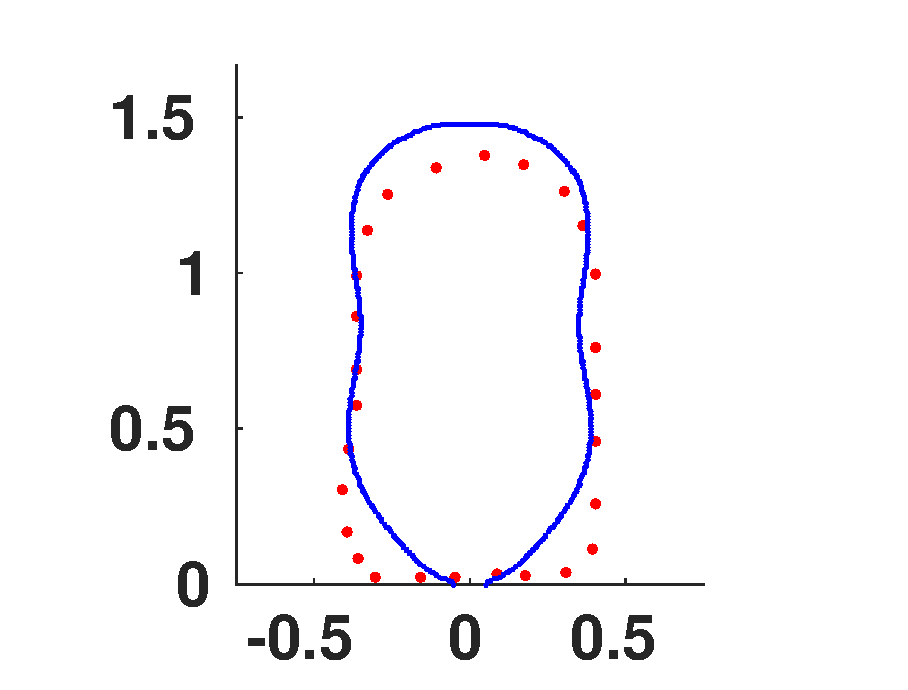
\includegraphics[width=0.3\textwidth]{wang-4.eps}
      }
    \subfloat[t = 19.0 ]{%
      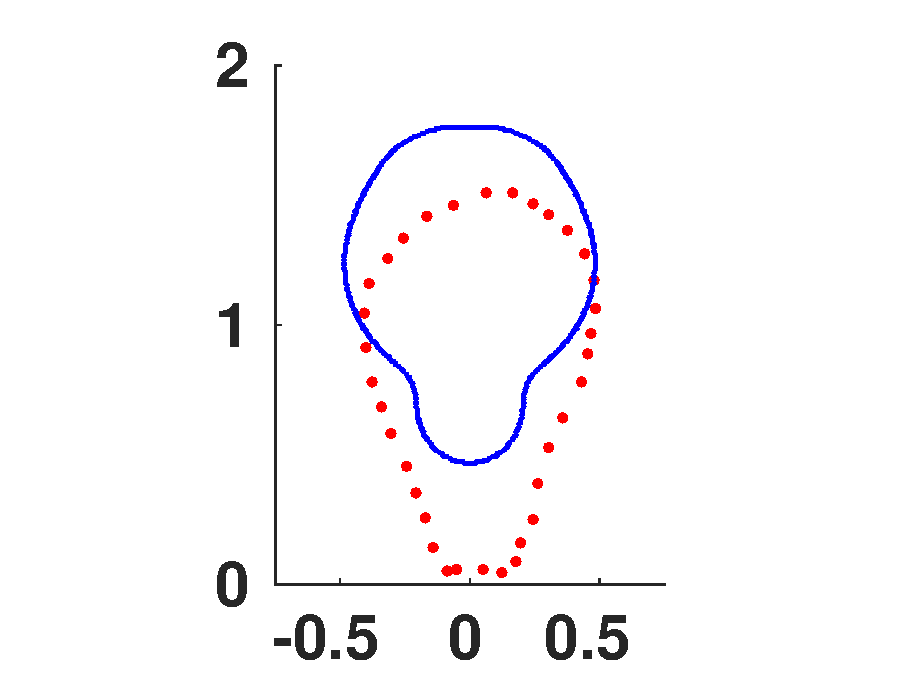
\includegraphics[width=0.3\textwidth]{wang-5.eps}
      }
       \subfloat[t = 19.5 ]{%
      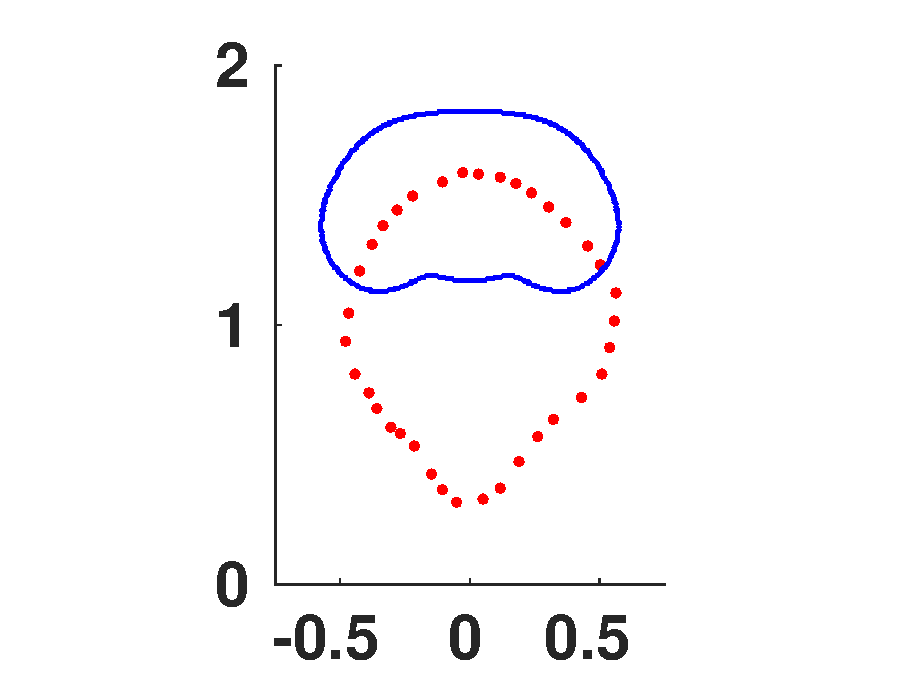
\includegraphics[width=0.3\textwidth]{wang-6.eps}
      }
    \caption{Interface Gerris simulation data(blue) with \cite{Wang2007} experimental data(red) Contact Angle $163^o$ }
 \label{Fig:gs7}
 \end{figure}   
%   \begin{figure}[H]
%  \centering
%  \subfloat[t = 15.6 ]{%
%       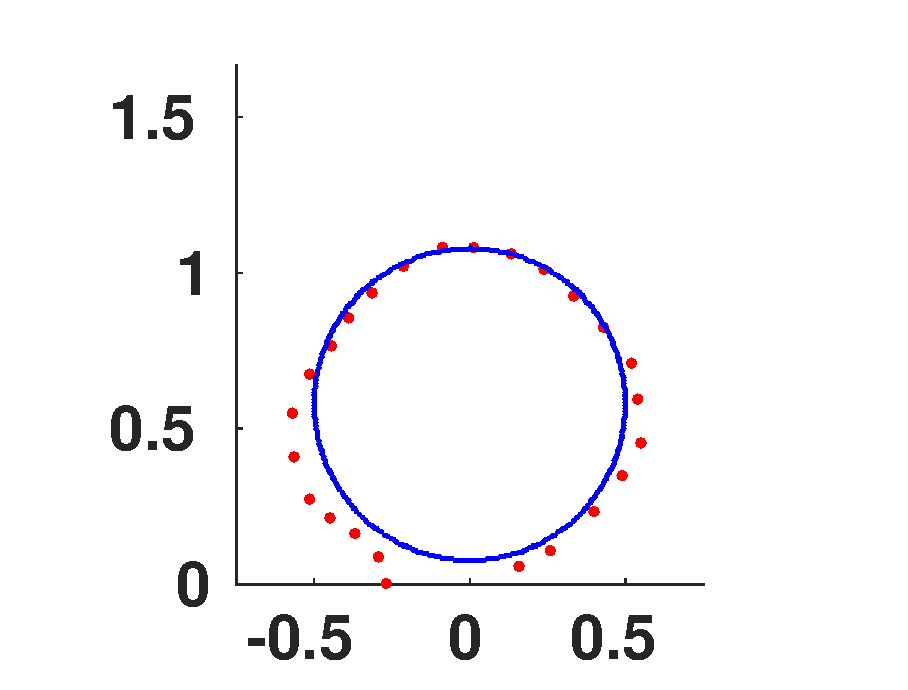
\includegraphics[width=0.3\textwidth]{wang-140-1.eps}
%       }
%   \subfloat[t = 16.6 ]{%
%       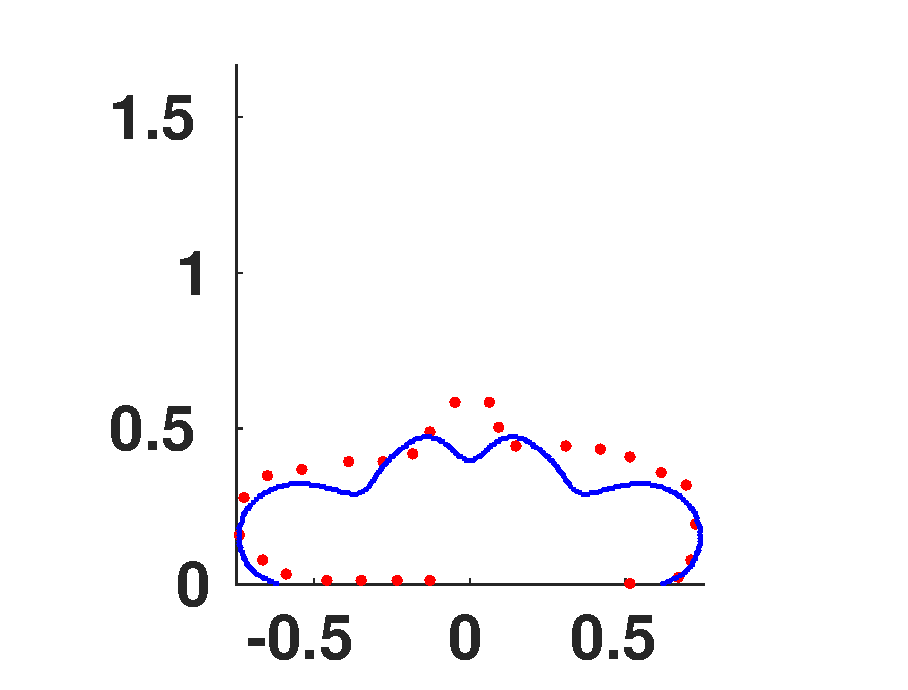
\includegraphics[width=0.3\textwidth]{wang-140-2.eps}
%       } 
%        \subfloat[t = 17.5 ]{%
%       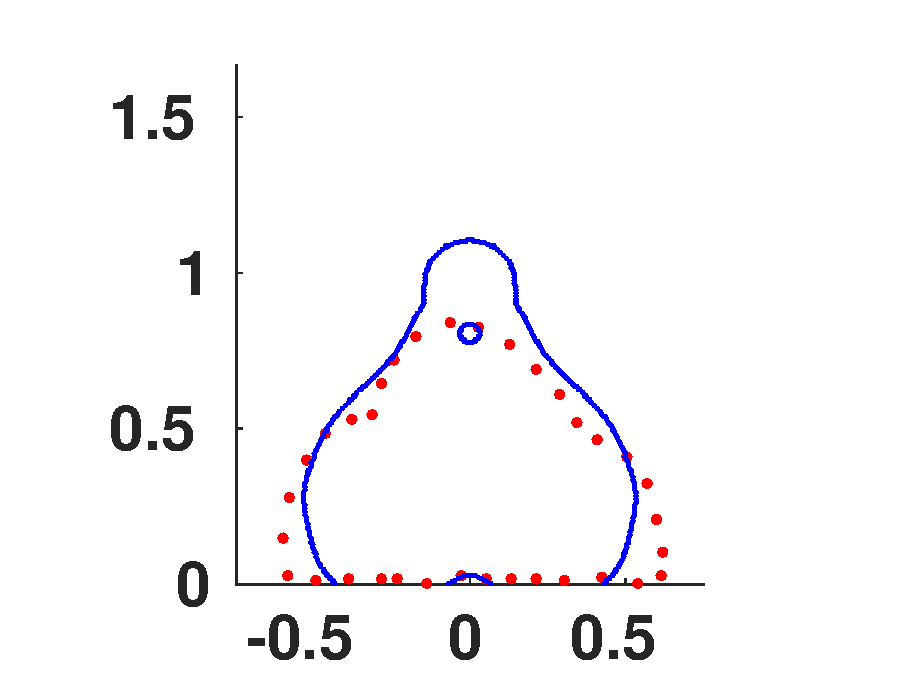
\includegraphics[width=0.3\textwidth]{wang-140-3.eps}
%       }\\
%        \subfloat[t = 20.4 ]{%
%       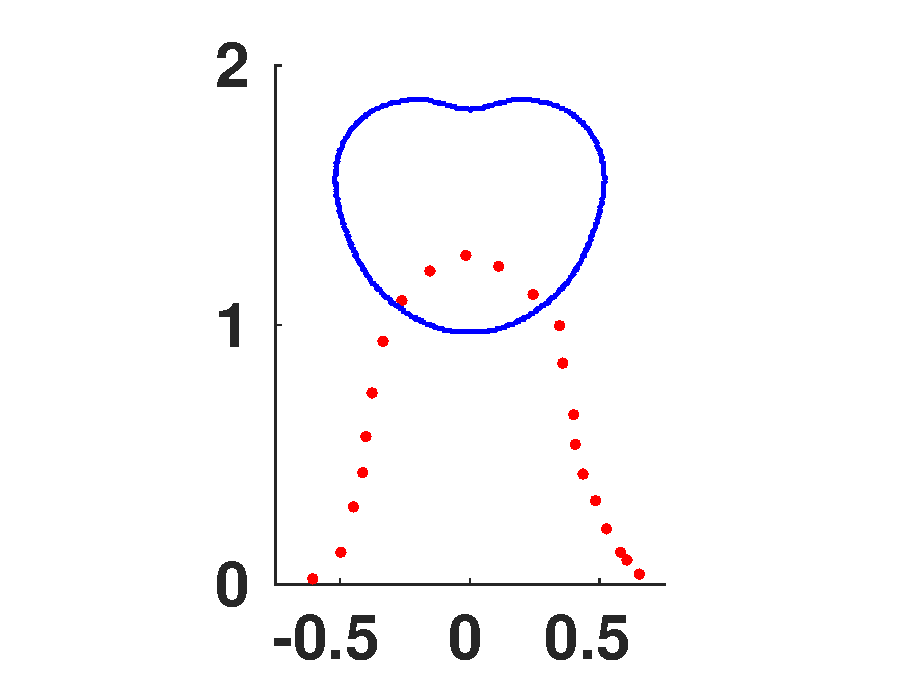
\includegraphics[width=0.3\textwidth]{wang-140-4.eps}
%       }
%     \subfloat[t = 21.9 ]{%
%       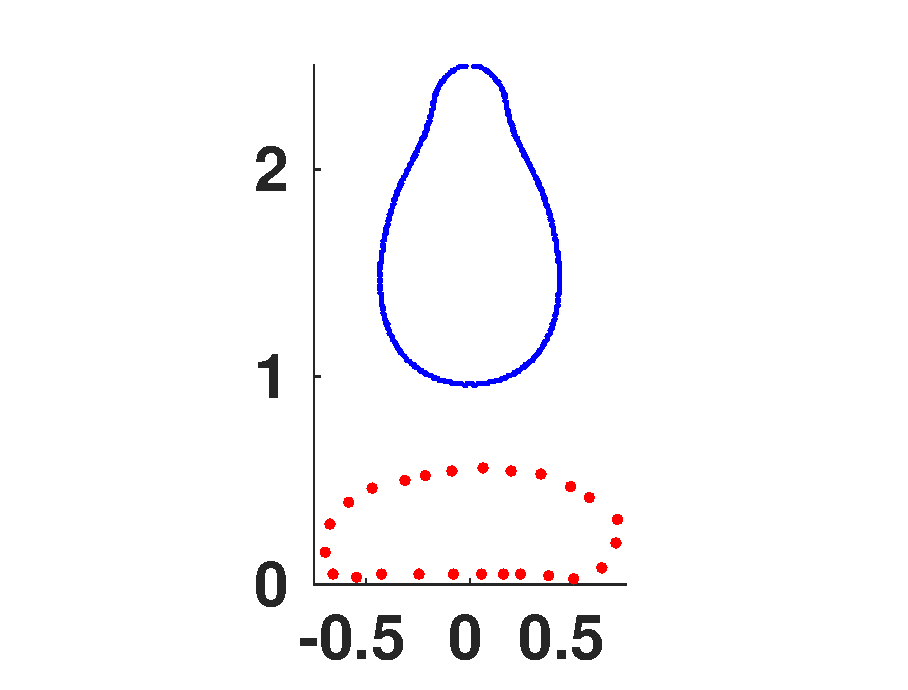
\includegraphics[width=0.3\textwidth]{wang-140-5.eps}
%       }
%        \subfloat[t = 24.6 ]{%
%       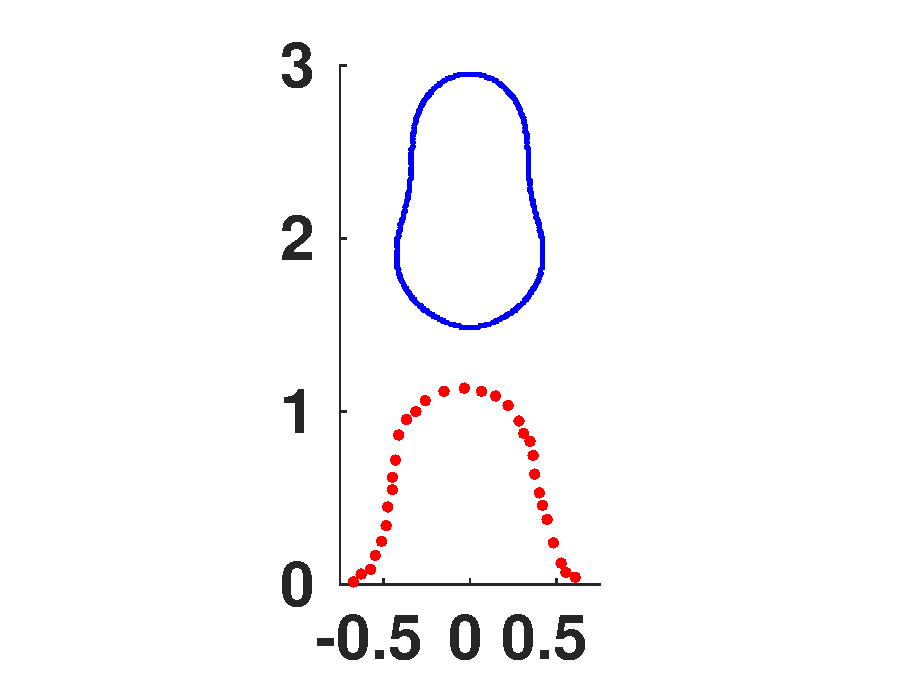
\includegraphics[width=0.3\textwidth]{wang-140-6.eps}
%       }
%     \caption{Interface Gerris simulation data(blue) with \cite{Wang2007} experimental data(red) Contact Angle $140^o$}
%  \label{Fig:gs8}
%  \end{figure}
\begin{figure}
 \centering
 \includegraphics{y_com_hung.eps}
 \caption{y coordinate of center of mass of droplet to time}
 \label{Fig:y_com}
\end{figure}

\section{Conclusion}
Preliminary data seems to suggest that the droplet dynamics and impact on superhydrophobic surfaces is not very sensitive to the precise nature of boundary conditions at the contact line.
Further studies are underway to validate this. Some directions of future research are indicated below:
\begin{enumerate}
\item Motion of center of mass of droplet. 
 \item Droplet impact on inclined plane.
 \item Droplet impact inclined to the plane.
 \item Oscillations of droplet after impact.
 \item Droplet breakup after impact.
\end{enumerate}
As Gerris does not have a dynamic contact angle model, we are in process of developing a multiphase Navier-Stokes solver and to implement 
the dynamic contact line model in it. Our code is expected to mimic droplet impact after implementation of contact model. We plan to explain
some aspects of this phenomena through simple mathematical models.


% \begin{figure}
%  \centering
%  \subfloat[ ]{%
%       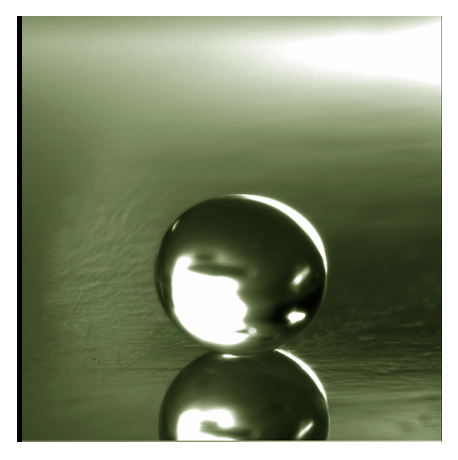
\includegraphics[width=0.3\textwidth]{droplet_c1.eps}
%       }
%   \subfloat[t = 27.1 ]{%
%       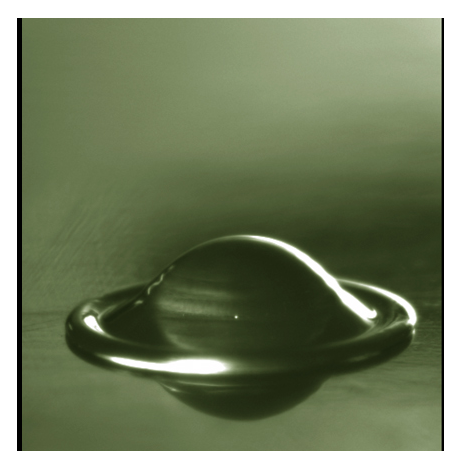
\includegraphics[width=0.3\textwidth]{droplet_c2.eps}
%       } 
%        \subfloat[t = 28.0 ]{%
%       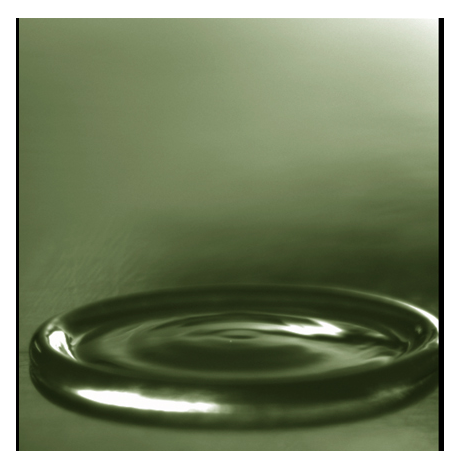
\includegraphics[width=0.3\textwidth]{droplet_c3.eps}
%       }
%   \caption{Moving contact line during impact}
%   \label{Fig:contact_line}
%   \end{figure}
